\section{Conclusion}

Decentralized systems are inherently more reliable, resilient against brute force attacks, and are more transparent. Fulfillment of smart contracts is limited due to off-chain information, logistical challenging obtaining impartial or truthful inputs from stakeholders, and verification of transaction completion involving real-world assets. This suggests effectiveness of smart contracts is currently limited to digital assets rather than for physical assets.  In addition, translating legal-binding contracts to code is challenging because the majority of programmers lack a legal background.

\begin{figure}[H]
\centering
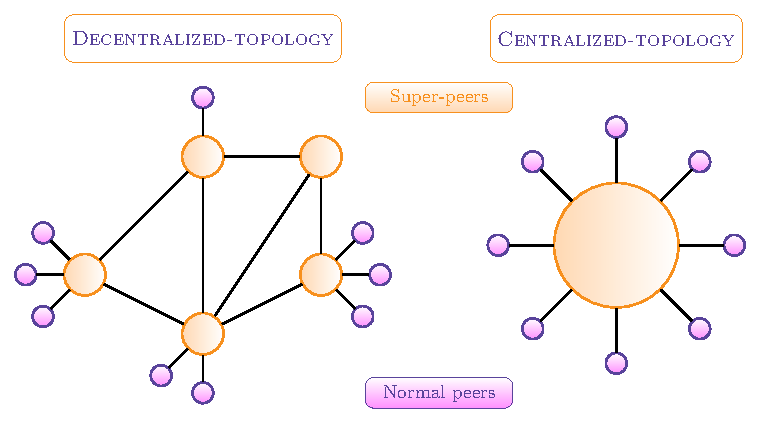
\includegraphics[width=0.5\linewidth]{Diagrams/DappVApp}
\caption{Decentralized structure vs Centralized Structure}
\label{fig:dappvapp}
\end{figure}

Despite shortcomings that involve transactional steps that are computational impossible to verify (package is delivered), performance of smart contracts is superior as transactions are tamper-proof.
Additionally, reduction of ambiguity from usage of smart contracts is highly probable because only one interpretation is possible. Coding errors or bugs exist in every non-trivial application, therefore transactions through smart contracts intrinsically carry some risk. This implies protocols and prior real-world agreements are necessary to migrate risk when executing smart contracts. Furthermore, increased precision and detail for transactional inputs and outputs required for creating smart contracts would benefit all parties. 

As shown in Figure \ref{security:fig2} only computers with significant high processing power  (quantum computers) can decrypt a 256 bit ethereum key cost-effectively. This indicates trying to hacking private keys is not a worthwhile venture.
Overall, smart contracts in conjunction with blockchain technologies allow for users to have a unique digital presence, securely transfer ownership of assets and avoid key shortcomings of centralized IT systems.

\newpage
%Despite Even though immutable and irreversible transactions are advantageous, criminals leverage cryptocurrencies for illegal transfer of funds. %This implies the ability to undo fraudulent or criminal activity is extremely important, but reversible transactions is an anti-pattern. %For example EOS, a centralized blockchain platform, was criticized for freezing accounts without due process and community backing. \cite{EOS:Online}. In addition, centralized systems require users to trust vendors and oftentimes personal data usage lacks transparency. Currently, research into blockchain technologies are actively researched that can disrupt existing industries including finance, real-estate and supply chains. \hfill \break
% 

%Deployment of a smart contract is inexpensive, however, development and maintenance costs for blockchain applications can be costly. This implies that transaction expenses decrease significantly, but running a blockchain node, ensuring high quality code for smart contracts is challenging and expensive. Decentralized applications are transparent because information is available in the publicly ledger and parties participating in a transaction cannot alter it. Overcomplicated code and bugs in smart contracts are severely detrimental because of malicious transactions by scammers or hackers. \hfill \break


%Smart contract reduce complexity of transactions allowing buyers to directly interact with sellers. This illustrates how useful smart contracts are, but lack of legislation for blockchain technologies, consortiums unwilling to adopt decentralized applications (may prefer private blockchains), and ability for hackers to exploit bugs suggest transactions governed by code is decades away. Solutions to existing problems in blockchain technologies such as latency, immutable transactions and widespread acceptance by consortiums are addressed through innovations such as sidechains, centralized blockchain platforms like EOS and private blockchains infrastructure. \hfill \break
